\section{Specifications}
\label{sec:Specifications}

\newcounter{rulei}[subsection]
\newcommand{\rcnii}{\stepcounter{rulei}\arabic{section}.\arabic{subsection}.\arabic{rulei}}
\renewcommand{\labelenumi}{\rcnii}

\subsection{Markers}
\label{sub:markers}
The arena, tokens and robots involved in the game are labelled with \textit{libkoki} markers.
Each marker pattern encodes a number.
Each marker number is associated with a particular feature within the arena, and also has an associated size.
The marker numbers and sizes are as follows:

\begin{center}
  \begin{tabular}{lcc}
    \toprule
    \textbf{Item} & \textbf{Marker Numbers} & \textbf{Marker Size (mm)} \\
    \midrule
    % Don't use marker 131: https://github.com/srobo/libkoki/issues/5
    Arena boundary & {} 0 -- 27 & 250 \\
    Gold tokens & {} 32 -- 39 & 250 \\
    Silver tokens & {} 40 -- 47 & 250 \\
    \bottomrule
  \end{tabular}
\end{center}

Two sets of marker codes will be used: one for development purposes, and one for the competition itself.
The competition set is only to be used inside the Student Robotics arena at the Student Robotics competition.
This is so that people carrying markers past the arena do not confuse robots.
The competition codes are 100 above the development codes.
When run in competition mode, the software provided by Student Robotics will subtract 100 from the detected marker codes, as well as ignore the development codes.

The markers can be printed on a black-and-white printer.
Marker designs can be downloaded from the documentation section of the Student Robotics website.

Unless specified otherwise, all markers described in this document are oriented vertically such that the principle corner of the marker (which is indicated by a dark grey dot in the black marker border) is on the higher edge.

\subsection{Robot Flag}
\label{sub:robot-flag}

\begin{figure}
  \centering
  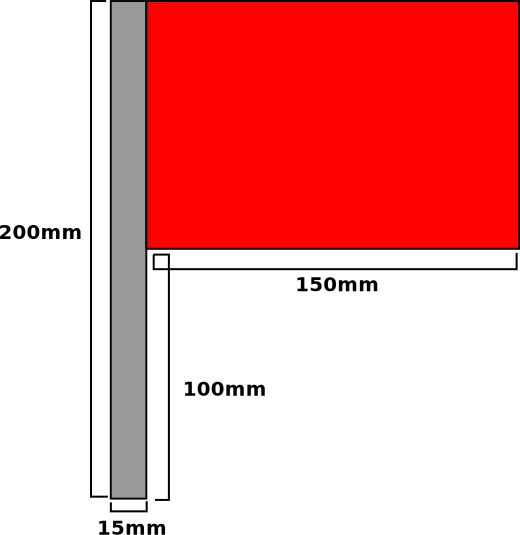
\includegraphics[width=0.5\textwidth]{./images/robot-flag.pdf}
  \caption{An example robot flag.}
  \label{fig:example-flag}
\end{figure}

\begin{enumerate}
  \item A ``robot flag'' is a removable identifier that will be attached to a robot throughout a match.
        It features identifying areas to allow spectators to easily associate a robot with its starting area.
        An example of one of these flags is shown in figure~\ref{fig:example-flag}.
        The markings in the identifying areas are intentionally not specified.

  \item Robot flags will be mounted on cylinders with a diameter of $15mm\pm1mm$,
        and a length of $200mm\pm10mm$.

  \item The identifying area will be attached to the top $100mm\pm10mm$ of the mounting cylinder,
        with a width of $150mm\pm10mm$, as described in figure~\ref{fig:example-flag}.

  \item The mounting cylinder must be permanently affixed to the main chassis of a robot, and vertical
        when the robot is in its typical stopped position.

  \item The identifying part of the robot flag must be visible when attached to the mount.

  \item Flags are not counted when considering the starting size of the robot.
\end{enumerate}

\subsection{Arena}
\label{sub:arena}
\begin{enumerate}
\item The match arena floor, overall, is an $8m \times 8m$ square, as shown in figure~\ref{fig:arena-dim}.
      The tolerance of these two dimensions is $\pm0.2m$.

\begin{figure}
  \centering
  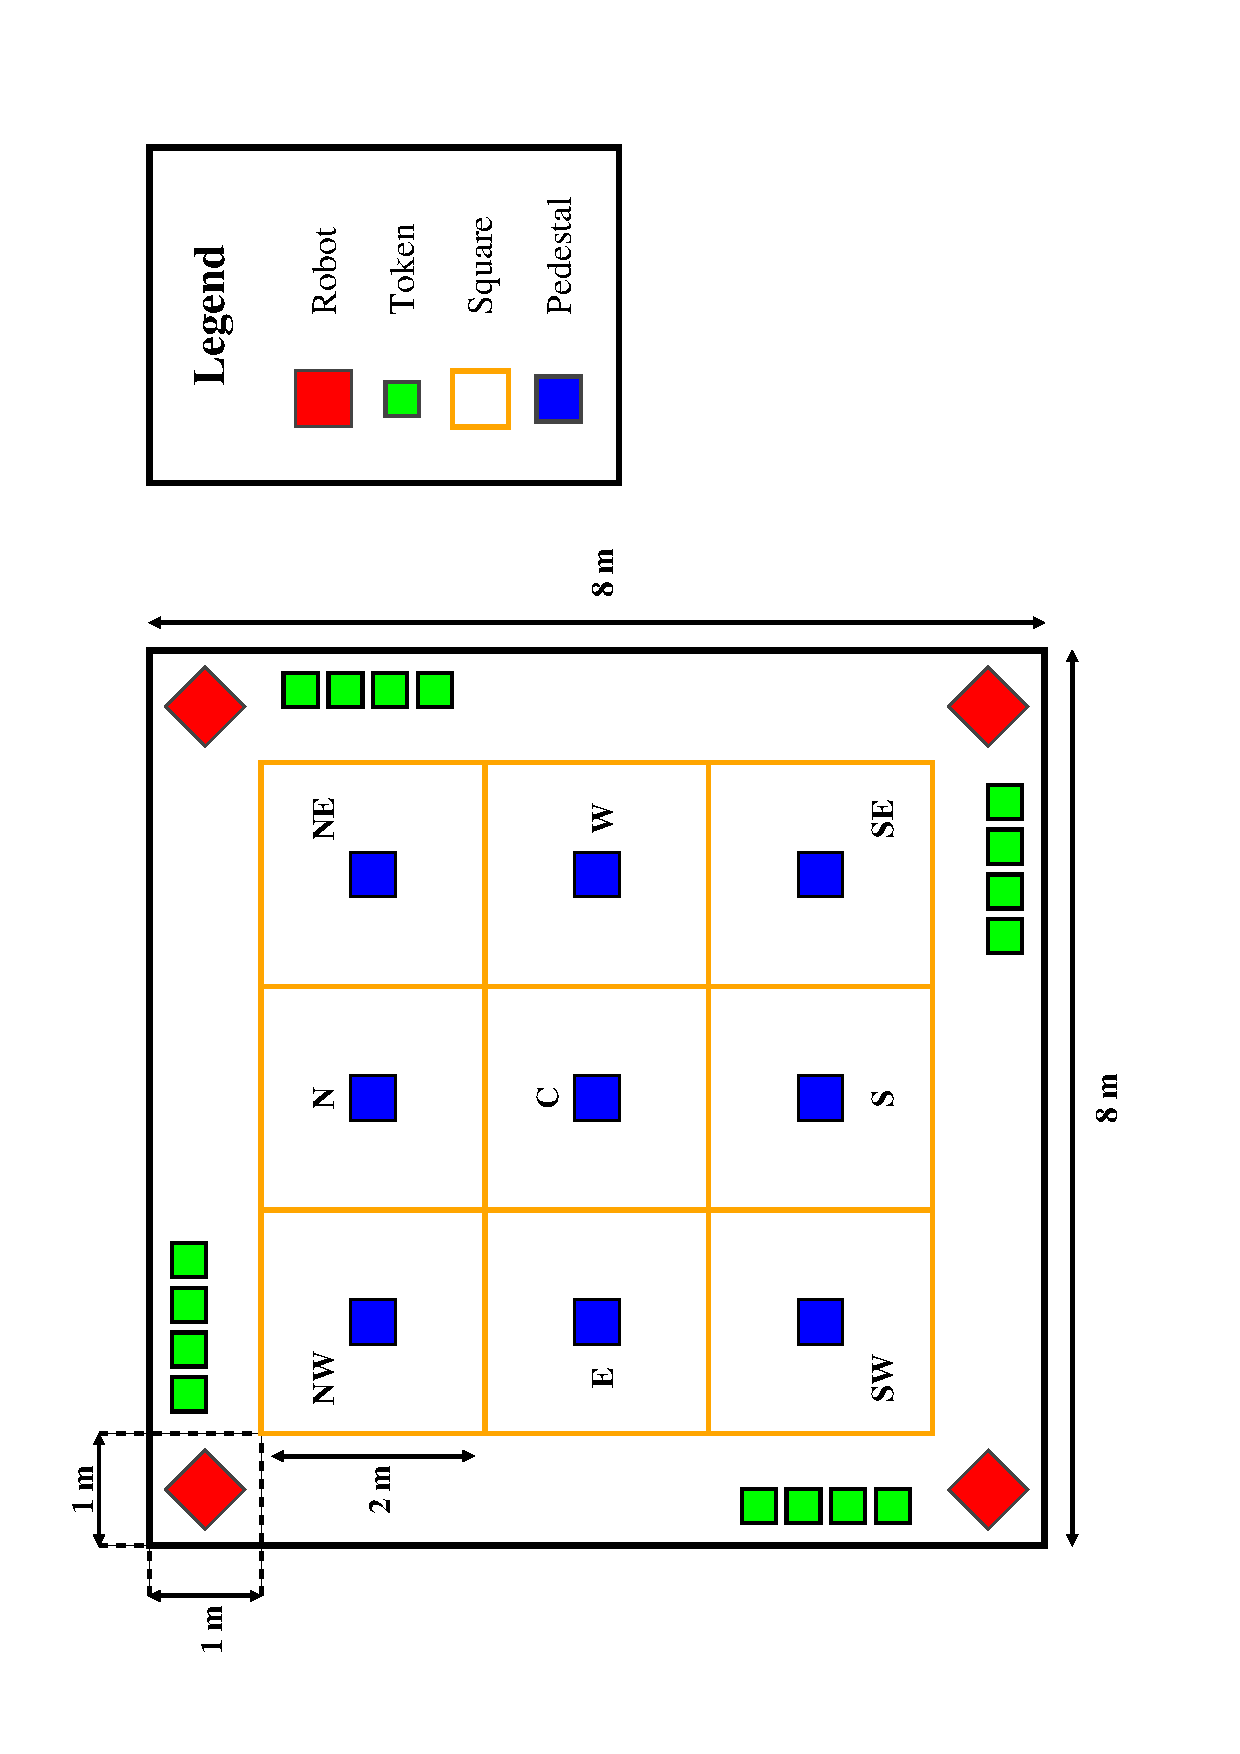
\includegraphics[width=\textwidth]{./images/arena.pdf}
  \caption{\label{fig:arena-dim}A bird's-eye view of the arena. All dimensions are in millimetres.}
\end{figure}

\item The floor of the arena is covered with a closed-loop, short pile carpet.

\item The perimeter of the arena floor is delimited by the arena wall, which has a minimum height of $100mm$.

\begin{figure}
  \centering
  
\includegraphics[width=\textwidth]{./images/sidewall.pdf}
  \caption{Seven $250mm$ wide markers are spaced evenly along each $8m$ arena wall.
           The markers are placed $50mm$ above the floor.
           All dimensions are in millimetres.}
  \label{fig:arena-wall}
\end{figure}

\begin{figure}
  \centering
  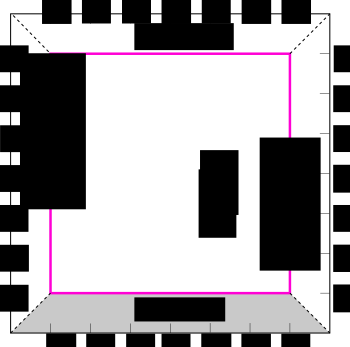
\includegraphics[width=0.5\textwidth]{./images/arena-markers.pdf}
  \caption{Twenty eight arena wall markers are positioned around the perimeter of the arena with the marker codes incrementing in a clockwise fashion.
           The corners are counted in a clockwise fashion, with corner 0 being the corner closest to arena marker 0.}
  \label{fig:arena-zones}
\end{figure}

\item Each wall of the arena features seven $250mm$ libkoki markers.
      Figure~\ref{fig:arena-wall} shows the positioning of these markers, whilst figure~\ref{fig:arena-zones} shows the numbering of these markers.

\item Each robot will be assigned a corner at the start of every match to indicate its starting area.
      Corner starting areas are $1000 \pm 20mm$ square and will be marked by tape.
      The mapping of these corner numbers in the arena is shown in figure~\ref{fig:arena-zones}.

\item Student Robotics reserves the right to have match officials in the arena during games.

\item In the centre of the arena is a raised area of height with $180 \pm 20mm$ a side length of $1200 \pm 100 mm$.

\end{enumerate}


\subsection{Scoring Zones}
\label{sub:Zones}

\begin{enumerate}
\item The four scoring zones form right-angled triangles, with the right angle described by the corner of the arena and the short sides of length $3000mm \pm 50mm$.
      The arrangement and dimensions of these zones can be seen in figure~\ref{fig:arena-dim}.

\item Edges of scoring zones will be marked by $48mm$ coloured tape.
      The tape will be placed along the inside of the edge of the zone, including it in the zone for scoring purposes.
\end{enumerate}

\subsection{Tokens}
\label{sub:Tokens}
\begin{enumerate}
\item Tokens are cubic cardboard boxes with a side length of $250 \pm 20 mm$.

\item Tokens will be arranged as shown in figure~\ref{fig:arena-dim} at the start of a match.

\end{enumerate}

\clearpage
